\documentclass[11pt]{article}

\usepackage[margin=1in]{geometry}
\usepackage[T1]{fontenc}
\usepackage{newtxmath}
\usepackage{graphicx}
\usepackage{float}
\usepackage{tikz}
\usetikzlibrary{positioning,arrows.meta,shapes.multipart,fit,backgrounds,calc,patterns}
\usepackage{booktabs}
\usepackage{array}
\usepackage{longtable}
\usepackage{xcolor}
\usepackage{listings}
\usepackage{hyperref}
\usepackage{caption}
\usepackage{enumitem}
\usepackage{amsmath}
\usepackage{fancyhdr}
\usepackage{titlesec}
\usepackage{microtype}
\usepackage{parskip}
\setlength{\emergencystretch}{3em}
\linespread{1.08}
\setcounter{secnumdepth}{3}
\setcounter{tocdepth}{3}

\hypersetup{
  colorlinks=true,
  linkcolor=blue!50!black,
  citecolor=blue!50!black,
  urlcolor=blue!50!black,
}

\lstdefinestyle{hex}{
  basicstyle=\ttfamily\small,
  columns=fullflexible,
  breaklines=true,
}

\pagestyle{fancy}
\fancyhf{}
\fancyhead[L]{\small Veritas86: Do We Trust Silicon? (Mid-Semester Report)}
\fancyhead[R]{\small \thepage}
\renewcommand{\headrulewidth}{0.3pt}

\titleformat{\section}{\normalfont\Large\bfseries}{\thesection}{1em}{}
\titlespacing*{\section}{0pt}{2.2em}{1em}
\titleformat{\subsection}{\normalfont\large\bfseries}{\thesubsection}{1em}{}
\titlespacing*{\subsection}{0pt}{1.6em}{0.8em}
\titleformat{\subsubsection}{\normalfont\bfseries}{\thesubsubsection}{0.7em}{}
\titlespacing*{\subsubsection}{0pt}{1.3em}{0.5em}

\newcommand{\code}[1]{\texttt{#1}}
\newcommand{\project}{Veritas86}

\title{\textbf{Veritas86: Do We Trust Silicon?}\\[4pt]
\large A Black-Box x86 Silicon Auditor, Motivated by the Hardware Trust\\[2pt]
\large Assumptions Beneath Cryptographic Guarantees}
\author{Aman Pathak \\ \small \texttt{p20260018@goa.bits-pilani.ac.in} \\ \small \url{https://github.com/vajradevam/veritas86}}
\date{Mid-Semester Report, October 14, 2026}

\begin{document}
\maketitle

\begin{abstract}
Cryptography is a necessary condition for security, not a sufficient one:
a correct algorithm proves nothing about the system that runs it, and the
security literature has made this point since at least Anderson's survey
of real-world cryptosystem failures \cite{anderson1993} and Kocher's
demonstration that a mathematically sound implementation can leak its own
key through timing alone \cite{kocher1996}. Underneath every
implementation sits hardware, and a general-purpose processor executes
cryptographic primitives, including hardware-accelerated AES, as opaque
silicon whose documentation describes intended behavior without
guaranteeing it \cite{thompson1984}. This report takes cryptography as its
entry point and then goes further: the tool built for this project,
\project{}, is not a cryptography-specific checker but a general-purpose,
black-box, ring-3 instruction fuzzer, and the bulk of this report is
results from pointing it at the fleet's entire reachable instruction
surface, not only the instructions that happen to be cryptographic.
Three sweeps are reported, growing from 823 to 2{,}689 to 4{,}996
candidates under two input states, across a fleet that grew from four to
six real machines spanning five Intel microarchitecture generations
(Sandy Bridge-EP, Haswell, Kaby Lake-R, Coffee Lake, Tiger Lake), for
59{,}952 data points in the final sweep. The harness reproduces the
original sandsifter paper's headline finding, finds and fixes three real
safety gaps in its own code, and uses a second input state to show that
86\% of one ambiguous fault bucket was a measurement artifact rather than
a privilege signal. On the cryptography side, scalar AES-NI and
PCLMULQDQ are confirmed present on every machine in the fleet back to
2012, while their vectorized forms (VAES, VPCLMULQDQ, and AVX-512
\code{vaesenc}) are confirmed present on exactly the two 2020 machines,
and the RDRAND/RDSEED hardware-RNG boundary is pinned to the exact pair
of machines that sit on either side of it. On the security side, UMIP
and PKU, two kernel/CPU-enforced mitigations, are detected purely from
\code{\#UD}-versus-executes behavior, without the use of \code{cpuid}. Beyond
cryptography and security specifically, the same harness reconstructs a
19-feature support matrix and an 8-feature generational timeline across
the fleet of hardware we have, from fault behavior alone, demonstrating that the tool audits
silicon in general, with cryptography and security as its motivating but
not limiting case.
\end{abstract}

\newpage

\tableofcontents

\newpage

% ======================================================================
\section{Introduction}
% ======================================================================

A cryptographic primitive is a mathematical object. Security is a
property of a system, and a system is built from implementations,
protocols, and hardware. A proof about the mathematical object says
nothing about it directly. Anderson's survey of real-world cryptosystem
failures found that the overwhelming majority had nothing to do with weak
algorithms, and everything to do with how those algorithms were deployed.
Like wrong threat models, protocol-level mistakes, and implementation bugs
\cite{anderson1993}. Kocher showed something more important, that is, an
implementation of RSA, Diffie-Hellman, or DSS can be algorithmically
unbroken and still hand an attacker the secret key, because the time the
implementation takes to run depends on the key, and that timing channel
exists entirely outside the mathematics being implemented
\cite{kocher1996}. Schneier made the general version of the point
explicit by saying that cryptography is a branch of applied mathematics, and treating a
cryptographic primitive as a security solution by itself, rather than as
one component that security engineering has to be built around, is a
recurring and well-documented mistake \cite{schneier1998}. Cryptography
is, in short, a necessary condition for security. It is not a sufficient
one.

Every implementation eventually runs on hardware, and that is where the
chain of trust gets harder to inspect, instead of being easier. A modern
general-purpose processor is a black box which takes in bytes and
architectural state and produces results. This also includes the results of
instructions that exist specifically to accelerate cryptography, such as
AES-NI and its vectorized successors. The vendor's architecture manual
describes what those instructions are supposed to do. It does not (in fact it is actually impossible to do so) serve as proof that a given physical chip does only
that and nothing else. Ken Thompson's Turing Award lecture made the
underlying argument explicit decades ago, where he said, trust that is placed in a tool
cannot be verified by reading that tool's own documentation or even its
own source, because the thing being trusted is exactly the thing capable
of lying about itself \cite{thompson1984}.

For hardware specifically, this is not a hypothetical concern. King et
al.\ demonstrated that small, targeted hardware modifications can grant
an attacker privilege escalation while leaving a chip's documented
functional behavior untouched \cite{king2008}, and Becker et al.\ showed
that such modifications can be made at the dopant level, invisible to
optical inspection and to every standard verification process
\cite{becker2013}. No malicious intent is required to see the same gap:
Kocher et al.\ and Lipp et al.\ showed that ordinary, non-malicious
speculative-execution hardware, present in essentially every modern
processor, routinely behaves in ways its own architecture manual does
not describe, and that this undocumented behavior is directly
exploitable across privilege and process boundaries
\cite{kocher2019spectre, lipp2018meltdown}. Closest to the present work,
Moghimi's Downfall disclosed that Intel's AVX-512 gather instructions,
used among other things to accelerate cryptographic workloads, leak data
across security boundaries through a hardware optimization that the SDM
never mentions \cite{moghimi2023downfall}.

In every one of these cases, the manual was not wrong in what it
claimed. It was silent about the part of the hardware's actual behavior
that mattered. That silence is the gap this report measures.

\subsection{Scope: cryptography as an entry point, not a boundary}
\label{sec:scope}

This report uses cryptography as its motivating entry point, because
"can I trust the AES-NI instruction this program is about to run" is a
concrete, well-posed version of the much larger question "can I trust
this silicon," and because the security literature above gives it a
precise theoretical frame. The tool built to answer it, \project{}, does
not stop at cryptography. It is a general-purpose, black-box, ring-3
instruction fuzzer to which given any byte sequence and any input register state,
it reports what the CPU actually did, with no assumption that the
sequence is cryptographic, privileged, or otherwise special. The bulk of
this report, Sections~\ref{sec:result-crypto} through
\ref{sec:result-silicon-map}, reflects that scope directly: after the
cryptography-specific results, the same unmodified harness is pointed at
the fleet's general instruction surface and recovers a 19-feature support
matrix and an 8-feature generational timeline (Figures~\ref{fig:matrix}
and \ref{fig:timeline}) that have nothing to do with cryptography
specifically, covering everything from AVX2 and BMI to memory-ordering
instructions and reserved opcode space. Cryptography motivates the
project. It does not define the tool's boundary.

Christopher Domas's 2017 Black Hat talk and whitepaper, \emph{Breaking
the x86 Instruction Set} \cite{domas2017}, gave this problem a concrete,
reproducible methodology: \emph{sandsifter}, a ring-3 fuzzer that uses
page-fault boundary detection to measure the true length silicon assigns
to an arbitrary byte sequence, independent of what any disassembler or
manual predicts. This project, \project{}, takes that methodology as a
starting point and reimplements its core technique in modern C: ring-3
single-step execution, guard-page length resolution, and signal-based
fault classification. It then asks a question scoped specifically to the
trust problem laid out above, using the hardware actually available for
this work. Given a fleet of ordinary, heterogeneous x86-64 machines,
including machines that implement hardware-accelerated cryptography, how
much can be learned about each one's actual behaviour, its silicon
generation, its security configuration, and whether its
cryptography-accelerating instructions are even present, purely from
black-box instruction-level observation, with no privileged access and
no use of \code{cpuid}?

The results reported here go further than expected. Beyond reproducing
the original paper's calibration result, cross-machine fingerprinting
recovers CPU generation boundaries cleanly, including the boundaries of
AES-NI, SHA-NI, GFNI, RDRAND, and RDSEED support, and recovers whether
UMIP and PKU, two kernel/CPU-enforced security mitigations, are active on
a given machine, entirely from fault-class patterns. None of this
required reading a single byte of \code{cpuid} output. It is exactly the
kind of fact a cryptographic system depends on silently and cannot verify
about itself from inside its own process.

\subsection{Research Questions}
\begin{enumerate}[label=\textbf{RQ\arabic*}.]
  \item Does a from-scratch, modern reimplementation of the sandsifter
    technique reproduce the original paper's headline divergence on
    current silicon? (\S\ref{sec:result-correctness})
  \item How much of the one- and two-byte x86 opcode space is identical
    across independent silicon implementations of the same architecture,
    and how much diverges as the corpus is deliberately widened across
    three successive sweeps? (\S\ref{sec:result-stability})
  \item Can microarchitectural feature boundaries, including the hardware
    cryptography instructions (AES-NI, PCLMULQDQ, SHA-NI, GFNI, RDRAND,
    RDSEED), AVX-512, BMI1/BMI2, and the security mitigations UMIP and
    PKU, be recovered from fault-class fingerprints alone, without
    \code{cpuid}? (\S\ref{sec:result-crypto}--\S\ref{sec:result-silicon-map})
  \item Does the same technique generalize beyond cryptography and
    security to a broad, general-purpose map of a fleet's silicon
    generation, without being re-targeted or redesigned for each new
    feature? (\S\ref{sec:result-silicon-map})
  \item What practical engineering hazards show up when running such a
    harness at scale, repeatedly, across heterogeneous real machines, and
    how should they be handled? (\S\ref{sec:result-bugs}, \S\ref{sec:result-sigbus})
\end{enumerate}

% ======================================================================
\section{Related Work}
% ======================================================================

\textbf{sandsifter} \cite{domas2017} is the direct ancestor of this
project. It is a Python 2 tool that walks candidate byte sequences, using
an unmapped guard page immediately after the candidate's execution buffer
to detect the exact number of bytes the CPU's instruction fetch unit
consumed, regardless of whether the resulting instruction turns out to be
valid, privileged, or undocumented. This project reimplements that
technique in modern C and adds \code{ucontext}-based state capture, which
the original injector did not have. The corpus construction is scoped
differently: rather than sandsifter's recursive ``tunneling'' search for
length anomalies, this project uses flat and systematic ModRM-level
enumeration of named opcode maps and instruction groups, together with
targeted, named feature seeds. That is enough to answer the research
questions above without requiring the XED or liblisa dependencies the
project's long-term plan calls for (see \S\ref{sec:limitations}).

\textbf{XED} (Intel's X86 Encoder Decoder) and \textbf{liblisa} are
reference decoders and instruction-semantics libraries that the project's
long-term design (\code{IMPLEMENTATION\_PLAN.md}) calls for as a
ground-truth oracle, to flag silicon or decoder divergences automatically
against documented semantics. Neither is wired in for the results in this
report. Every length and fault prediction here is empirical, compared
across machines rather than against a reference decoder. This is a
deliberate scope reduction, discussed further in \S\ref{sec:limitations}.

The broader motivation for treating this as a security question, not only
an ISA-archaeology one, comes from outside the systems literature named
above as much as from inside it: Anderson's and Kocher's results
establish that correctness of an algorithm is independent of the security
of a system built around it \cite{anderson1993, kocher1996}, and
Thompson's, King et al.'s, and Becker et al.'s results establish that a
hardware component's documentation cannot be treated as proof of its
behavior \cite{thompson1984, king2008, becker2013}. Put together, a
cryptographic guarantee that depends on a specific hardware instruction,
AES-NI being the clearest example, depends transitively on a claim about
silicon that the vendor's manual asserts but does not, and cannot, prove.
This project does not attempt to prove hardware correctness either;
empirical fuzzing cannot establish the absence of a backdoor. What it
does establish is a practical, repeatable method for catching the case
where documented and actual behavior disagree, which is a strictly weaker
but directly useful goal, and one that turns out to be achievable with no
privileged access at all.

\textbf{UMIP} (User-Mode Instruction Prevention) is documented in the
Intel SDM \cite{intelsdm}, Volume 3, \S2.5, as a \code{CR4} bit (bit 11)
that, when set, causes \code{sgdt}, \code{sidt}, \code{sldt}, \code{str},
and \code{smsw} to raise \code{\#GP} when executed at CPL~$>$~0, instead
of their normal, unprivileged behavior of returning table-address
information. \textbf{PKU} (Protection Keys for Userspace), also
documented in SDM Volume 3, governs \code{rdpkru}/\code{wrpkru} and is
used by language runtimes and sandboxes (V8, WebKit, and others) to
isolate memory regions within a single process without a syscall. Both
are gated by CPUID feature bits and, for UMIP, a \code{CR4} bit set by
the kernel. This report demonstrates that the presence of both can be
recovered purely from differential black-box fault behavior, without
reading \code{CR4} or \code{cpuid} at all.

% ======================================================================
\section{System Design}
% ======================================================================

\subsection{The Injector Abstraction}

The project is organized around one interface: submit a candidate
encoding together with an input register state, and get back a result.
This interface is implemented twice, in two layers that must agree with
each other: \code{core/injector/proto.h} in C, and
\code{orchestrator/tsfuzz/proto.py} in Python, mirrored field for field.

\begin{lstlisting}[style=hex]
struct job {
  uint8_t  enc[15]; uint8_t enc_len;   // candidate bytes, actual length
  uint8_t  mode;                        // LENGTH | EXECUTE | BOTH
  uint64_t gpr[16]; uint64_t rflags;    // input architectural state
};
struct result {
  uint8_t  length; uint8_t valid_length;
  uint32_t fault;             // UD / BOUNDARY_PF / GP_OR_PF / FP / BUS / NONE
  uint64_t cr2_off;           // fault address, relative to exec_page base
  uint64_t gpr[16]; uint64_t rflags;    // output architectural state
  uint64_t rip_off;           // post-attempt RIP, relative to exec_page base
};
\end{lstlisting}

A long-lived C daemon (\code{core/injector/injector}) speaks this
protocol over a pipe to a Python driver (\code{Ring3Injector}), which is
the only backend implemented and the one used to produce every result in
this report. The design anticipates additional backends for future work:
QEMU-TCG, KVM ring-0, bare-metal ring-0, and RTL simulation
(\S\ref{sec:future}). None of those are built yet.

\subsection{How This Finds Hidden, Undocumented Behavior}
\label{sec:engine}

The method follows the same logic Domas used to break the x86 decoder in
sandsifter~\cite{domas2017}: do not start from the instructions the
manual says exist, because the manual is exactly the thing being
checked. Start from the raw byte space instead, ask the silicon itself
what each byte string does, and only then compare the answer against the
documentation. Anywhere the two disagree is either a bug in this
harness or a piece of real, previously hidden decoder behavior, and
every disagreement in this report was run down until it was clearly one
or the other. The rest of this subsection walks through exactly how a
single candidate byte string is turned into that answer, in four steps:
how its length is discovered without ever decoding it, how its fault
behavior is classified, a worked numeric example of both, and how
repeating this across the whole opcode map and across six different
machines is what actually surfaces the undocumented cases.

\subsubsection{Step 1: a length oracle built from a page fault, not a decoder}

The engine never parses an encoding to find out how many bytes long it
is; that would require already knowing the rules the project is trying
to test. Instead it places candidate bytes at the very end of a mapped,
executable page and leaves the page immediately after it unmapped, and
lets the CPU's own front-end decoder answer the question by fetching
bytes until either it has enough to decode an instruction or it walks
off the mapped page and faults.

A \code{SIGSEGV} whose faulting address (\code{siginfo.si\_addr}, read
back through \code{ucontext\_t}) lands exactly on that boundary means
one thing and one thing only: the decoder's instruction-length
calculation, whatever it is, needed more bytes than were resident. It
is not a statement that the instruction is invalid; truncated, perfectly
valid instructions produce exactly this fault. This is the same
reasoning sandsifter uses to bisect instruction length without ever
implementing a decoder of its own, because the only decoder whose
opinion matters here is the one on the chip.

\subsubsection{Step 2: single-stepping and classifying whichever signal actually fires}

Decoding is one thing; executing is another, and ring 3 cannot be
allowed to execute a candidate that might turn out to be \code{SYSCALL}
or a segment-register load. So before the candidate ever runs, the
engine arms \code{RFLAGS.TF} (the trap flag) through a single planted
\code{POPFQ} byte placed immediately before it, which forces the CPU to
raise \code{SIGTRAP} after the very next instruction boundary rather
than running freely. Combined with the blacklist in
\S\ref{sec:safety}, this means every candidate either single-steps
exactly once or is never executed at all. Figure~\ref{fig:classify}
shows how the signal that actually arrives is turned into one of five
outcomes.

\begin{figure}[H]
\centering
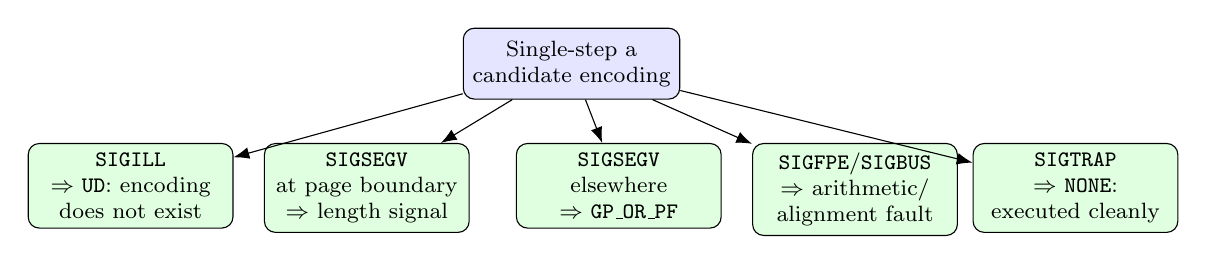
\begin{tikzpicture}[
  node distance=0.55cm and 1.0cm,
  box/.style={draw, rounded corners, align=center, font=\footnotesize, minimum width=2.6cm, minimum height=0.9cm},
  start/.style={box, fill=blue!10},
  leaf/.style={box, fill=green!12},
  arr/.style={-{Latex[length=2mm]}},
]
  \node[start] (sig) {Single-step a\\candidate encoding};
  \node[leaf, below=of sig, xshift=-5.6cm] (ill) {\code{SIGILL}\\$\Rightarrow$ \code{UD}: encoding\\does not exist};
  \node[leaf, below=of sig, xshift=-2.6cm] (segb) {\code{SIGSEGV}\\at page boundary\\$\Rightarrow$ length signal};
  \node[leaf, below=of sig, xshift=0.6cm] (segg) {\code{SIGSEGV}\\elsewhere\\$\Rightarrow$ \code{GP\_OR\_PF}};
  \node[leaf, below=of sig, xshift=3.6cm] (fpe) {\code{SIGFPE}/\code{SIGBUS}\\$\Rightarrow$ arithmetic/\\alignment fault};
  \node[leaf, below=of sig, xshift=6.4cm] (trap) {\code{SIGTRAP}\\$\Rightarrow$ \code{NONE}:\\executed cleanly};

  \draw[arr] (sig) -- (ill);
  \draw[arr] (sig) -- (segb);
  \draw[arr] (sig) -- (segg);
  \draw[arr] (sig) -- (fpe);
  \draw[arr] (sig) -- (trap);
\end{tikzpicture}
\caption{Fault classification from a single signal-handler invocation.
Every outcome is observed, not assumed; the handler runs on an
alternate signal stack and restores architectural state afterward so
the engine can move on to the next candidate regardless of which branch
fired.}
\label{fig:classify}
\end{figure}

\subsubsection{Worked example: finding the length of a four-byte encoding}

Domas's paper makes this concrete with a worked byte sequence, and the
same demonstration applies directly here. Take the four-byte encoding
\code{66 0F 38 DB} (a \code{66}-prefixed three-byte opcode, the real
encoding family for scalar \code{AESIMC}, used in this report's own
corpus). The engine does not start by assuming the answer is four. It
submits the byte string with every window length from one byte up to
the full candidate, right-justified against the guard page each time,
and watches where the boundary signal stops firing.

\begin{figure}[H]
\centering
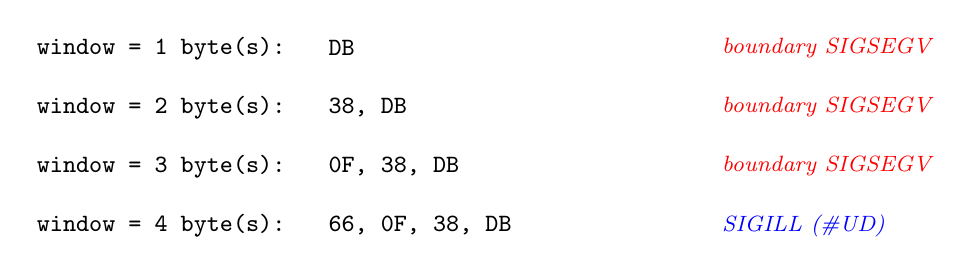
\begin{tikzpicture}[
  row/.style={font=\ttfamily\small},
  tag/.style={font=\footnotesize\itshape},
]
  \foreach \n/\bytes/\verdict/\tagcolor in {1/{DB}/{boundary SIGSEGV}/red,2/{38, DB}/{boundary SIGSEGV}/red,3/{0F, 38, DB}/{boundary SIGSEGV}/red,4/{66, 0F, 38, DB}/{SIGILL (\#UD)}/blue} {
    \pgfmathsetmacro{\y}{(4-\n)*0.75}
    \node[row, anchor=east] at (-0.3,\y) {window = \n{} byte(s):};
    \node[row, anchor=west] at (0,\y) {\bytes};
    \node[tag, text=\tagcolor, anchor=west] at (5.0,\y) {\verdict};
  }
\end{tikzpicture}
\caption{Length resolution for \code{66 0F 38 DB}, window by window. The
first three windows under-supply the decoder, which faults at the guard
page every time, a pure length signal. The four-byte window is the
first one the decoder can fully consume; it decodes to completion and
only then raises \code{SIGILL}, because this particular fleet member's
decoder does not implement \code{AESIMC} in this run's default state.
Resolved length: 4, independent of whether the instruction turns out to
exist.}
\label{fig:worked}
\end{figure}

The point this example is built to make is the same one sandsifter's
original write-up makes: the boundary fault at windows 1 through 3 says
nothing about whether \code{66 0F 38 DB} exists, only that the decoder
was not finished reading. Existence is answered separately, by whatever
signal fires once a full, un-truncated window is supplied, which is why
length resolution and fault classification are kept as two distinct
steps in this design rather than folded into one guess.

\subsubsection{Step 3: from a single answer to undocumented behavior}

A single classification for a single encoding is not yet a finding. Hidden
behavior becomes visible only once this length-and-fault oracle is run
over the entire byte space the Software Developer's Manual claims to
define, rather than only the mnemonics it names, and the result is
compared along two axes at once.

First, against the manual itself: every reserved or undefined region of
an opcode map (unused ModRM \code{reg} fields inside a group, unused
three-byte-map rows, prefix combinations the manual never discusses) is
swept with the same oracle as the documented mnemonics, because
undocumented behavior by definition will not be found by only trying
documented encodings. The 213-of-256 reserved-ModRM permissiveness
pattern in Group 7 (\S\ref{sec:result-silicon-map}) was found exactly
this way: nothing in the manual predicts that most of that group's
undefined space should fault as \code{GP\_OR\_PF} rather than
\code{UD}, and the only way to see that is to ask the silicon about all
256 ModRM values, not the handful the manual names.

Second, against the other five machines in the fleet. The same byte
string, run through the identical oracle on silicon from three
different microarchitecture generations, is expected by the manual to
decode identically wherever the manual's description does not depend on
a stated feature flag. When it does not, the disagreement is the
finding. The clearest example in this report is not a cryptography
instruction at all: EVEX-prefixed candidates (\code{0x62}) decode to
their full, correct 6--7 byte length on the two Tiger Lake and two
2017--2019 machines, and truncate to exactly 2 bytes on the Sandy
Bridge-EP and Haswell machines, because those two decoders do not
recognize \code{0x62} as an EVEX escape at all and instead read it as
the legacy, 64-bit-invalid \code{BOUND} opcode (\S\ref{sec:result-silicon-map}).
No CPUID flag the manual exposes documents that the \emph{byte}
\code{0x62} is interpreted two architecturally different ways depending
on silicon generation; this fell directly out of running the same
four-step process above on six machines side by side rather than one.

This is the same reasoning sandsifter is built around, applied here as
a general procedure rather than a one-off audit of a single CPU: the
length oracle and the fault classifier are each individually simple and
exhaustively applicable, and it is only their accumulation over the
full byte space, cross-checked against both the manual and a fleet of
real chips, that turns raw signal counts into a map of where the
documentation and the silicon disagree.

\subsection{Safety Design}
\label{sec:safety}

Every result in this report comes from ring-3 execution; no privilege
escalation is attempted anywhere in this work. A best-effort byte-pattern
blacklist (\code{core/injector/blacklist.c}) refuses to execute, though
it still permits length analysis of, encodings whose architectural
effect cannot be safely recovered from inside a signal handler. Three
such gaps were found empirically during this project, each by running
the harness at increasing scale, and each is covered in
\S\ref{sec:result-bugs}. The default input state zeroes every
general-purpose register except \code{RSP}, which points into the
scratch page, so that memory-operand instructions resolve into
disposable memory rather than the process's own live state. A preflight
script (\code{scripts/safety\_preflight.sh}) refuses to run as root
unless an explicit sacrificial-hardware flag is set. That flag was never
set for any result in this report; every machine in the fleet, including
the nominally sacrificial Xeon (z420), was used only in its normal, safe,
ring-3 mode.

\section{Experimental Setup}

\subsection{Fleet}
\label{sec:fleet}

Table~\ref{tab:fleet} lists the six machines used, connected over a
private Tailscale mesh network and accessed over SSH. All results in this
report were collected on 2026-10-14. The fleet grew across the course of
this work: the first sweep used four machines; the second added z420; the
third, reported here in full, added imac, a Haswell-generation machine
that fills the one generational gap the earlier Sandy-Bridge-EP-to-Tiger-
Lake comparisons could not resolve on their own (\S\ref{sec:result-silicon-map}).

\begin{table}[h]
\centering
\caption{Fleet used for this report, ordered by CPU release year.}
\label{tab:fleet}
\resizebox{\textwidth}{!}{%
\begin{tabular}{@{}llllr@{}}
\toprule
Host & CPU & Microarchitecture (year) & Microcode & OS/Kernel \\
\midrule
z420        & Xeon E5-1607 0      & Sandy Bridge-EP (2012) & 0x71a & Arch, 6.18.55-1-lts \\
imac        & Core i5-4570R       & Haswell (2013)         & 0x1c  & Arch, 6.18.55-1-lts \\
fuzzarch    & Core i7-8550U       & Kaby Lake-R (2017)     & 0xf6  & Arch, 6.18.55-1-lts \\
d153-system & Core i7-9700T       & Coffee Lake (2019)     & 0x104 & Ubuntu 24.04, 7.0.0-34-generic \\
lily        & Core i7-1165G7      & Tiger Lake (2020)      & 0xb6  & Arch, 7.2.2-arch1-1 \\
debian      & Core i7-1165G7      & Tiger Lake (2020)      & 0xbc  & Debian testing, 7.3.0-rc6+ \\
\bottomrule
\end{tabular}%
}
\end{table}

lily and debian share the identical CPU model, i7-1165G7, but run
different kernels and microcode revisions. This pair was kept
deliberately: it is the same-silicon control used in
\S\ref{sec:result-sigbus} to separate a kernel-specific bug from a
CPU-specific one.

\subsection{Three Sweeps}
\label{sec:corpus}

The corpus grew across three sweeps over the course of this project,
summarized in Table~\ref{tab:sweeps}. Each later sweep both widened
coverage and specifically targeted instruction groups likely to be
security- or cryptography-relevant: the third sweep added full
256-ModRM-byte sweeps of Group 7 (\code{0F 01}: PKU, TSX, SMAP, VMX,
\code{serialize}), Group 9 (\code{0F C7}: \code{cmpxchg8b/16b},
\code{rdrand}, \code{rdseed}), and Group 15 (\code{0F AE}) under three
more legacy prefixes (\code{clwb}/\code{clflushopt}/\code{tpause}/
\code{umwait}/\code{umonitor}); full \code{66}-prefixed and VEX-prefixed
three-byte-opcode-map sweeps (scalar and vectorized AES-NI and
PCLMULQDQ); and named seeds for AVX2/AVX-512 gather (the instruction
class at the center of Downfall \cite{moghimi2023downfall}) and
\code{rdpid}.

\begin{table}[h]
\centering
\caption{The three sweeps, in order.}
\label{tab:sweeps}
\begin{tabular}{@{}lrrrr@{}}
\toprule
Sweep & Candidates & Input states & Machines & Rows (total) \\
\midrule
1 & 823   & 1 & 4 & 823 \\
2 & 2{,}689 & 2 & 5 & 5{,}378 per machine (26{,}890 total) \\
3 & 4{,}996 & 2 & 6 & 9{,}992 per machine (59{,}952 total) \\
\bottomrule
\end{tabular}
\end{table}

All multi-byte instruction seeds requiring non-trivial encoding,
including the EVEX-prefixed AVX-512 instructions, the VEX-prefixed AES
and PCLMULQDQ forms, and the AVX2/AVX-512 gather seeds, were extracted
empirically rather than hand-assembled. A small C source file was
compiled with the corresponding \code{gcc} target flag (for example
\code{-mavx512f}, \code{-mavx2}, \code{-mpku}), and the resulting machine
code bytes were read directly from \code{objdump} output. This avoids the
class of bugs that comes from constructing VEX and EVEX prefix bytes by
hand.

\subsection{Input States}
\label{sec:states}

Every candidate in sweeps 2 and 3 was submitted under two named input
register states, to disambiguate a fault-class ambiguity discovered in
sweep 1 (\S\ref{sec:result-gppf}).

\begin{description}
  \item[\code{zero\_v1}] All GPRs are zero except \code{RSP}, which
    points into the scratch page. This has been the harness's default
    since the start of the project.
  \item[\code{scratch\_v1}] Every GPR, including \code{RSP}, is set to
    the same scratch-page pointer the daemon's handshake already
    guarantees is valid. This state is implemented entirely in Python
    (\code{orchestrator/tsfuzz/fingerprint.py}), with no change to the C
    engine, and is recomputed fresh from each daemon process's own
    handshake, never reused from a different process, since each daemon
    instance has an independent ASLR layout.
\end{description}

% ======================================================================
\section{Results}
% ======================================================================

\subsection{Engine Correctness: Known-Answer Tests}
\label{sec:result-correctness}

Before any sweep can be trusted, five known-answer cases
(\code{core/tests/smoke.c}) have to pass. They passed, 16 out of 16
assertions, on all six machines in the fleet, every time the engine was
rebuilt across all three sweeps. The headline case directly reproduces
the original paper's finding.

\begin{quote}
\code{66 E9 00 00 00 00} resolves to length \textbf{6} on every machine.
The \code{66} operand-size-override prefix is architecturally
meaningless on \code{jmp rel32} in 64-bit mode, so silicon decodes one
6-byte jump rather than a 2-byte jump followed by four stray bytes, which
is what a naive \code{66}-honoring disassembler would predict.
\end{quote}

\code{F4} (\code{hlt}) correctly reports that the encoding exists but
ring~3 cannot run it (\code{GP\_OR\_PF}), rather than \code{\#UD}, on
every machine. This confirms the harness can tell ``does not exist''
apart from ``exists, privileged,'' which the rest of this report depends
on.

\subsection{Three Real Safety Bugs Found and Fixed via Fuzzing}
\label{sec:result-bugs}

Running the harness at increasing scale against real, heterogeneous
machines found three distinct gaps in its own safety design, all of the
same general shape: an instruction whose architectural effect cannot be
safely recovered from inside a signal handler, missed by the blacklist
because it was not on any hand-picked list of ``known dangerous''
mnemonics.

\subsubsection{\code{pop fs}/\code{pop gs} (found in sweep 1)}

The first full two-byte-opcode-map sweep crashed the injector daemon
outright at \code{0F~A1} (\code{pop~fs}). The blacklist blocked
\code{mov~Sreg} and \code{lss}/\code{lfs}/\code{lgs} as segment-register
loads, but did not cover \code{pop~fs}/\code{pop~gs}
(\code{0F~A1}/\code{0F~A9}), which belong to the same hazard class
through a different opcode.

Loading \code{FS} from the sweep's zeroed GPR state breaks the
TLS-relative addressing that the process's own signal-handler
bookkeeping depends on, so the crash happens before the installed
handler can run at all. Fixed by adding both opcodes to the blacklist.

\subsubsection{\code{umonitor} (found in sweep 3)}

The full 256-ModRM sweep of Group 15 under the \code{F3} prefix killed
the daemon at every ModRM byte with
reg field \code{010} (\code{F3~0F~AE~D0}-\code{D7}, i.e.\
\code{umonitor}), on a \emph{single isolated job submitted to a freshly
started daemon with no prior state at all}, under either input state.

This rules out both explanations that would otherwise be the first
suspects. It is not the NULL-deref explanation that applied to the
\code{pop fs}/\code{gs} case, because it reproduces under
\code{scratch\_v1}, which points every GPR at valid memory. It is not an
accumulation effect either, because it is the very first job the daemon
ever processes. The daemon exits with Python's reported return code
$-11$, killed by a raw, uncaught \code{SIGSEGV}, despite \code{signals.c}
installing a handler for that signal; capturing the daemon's own
\code{stderr} across the crash shows that neither the handler's normal
result path nor its diagnostic for a signal arriving outside a
controlled attempt fired.

Fixed by extending the blacklist to track whether the \code{F3} prefix
specifically was present, and refusing \code{0F AE} when the ModRM byte
selects \code{mod=11, reg=010} under that prefix; the unprefixed and
\code{66}-prefixed forms of the same ModRM byte, already swept safely
elsewhere, are left alone.

\subsubsection{Both fixes, tested, and the lesson they share}

Both fixes are regression-tested, one test per bug
(\code{test\_blacklist\_refuses\_pop\_fs\_gs\_execute} and
\code{test\_blacklist\_refuses\_umonitor\_execute}
respectively), and the second test explicitly asserts the
unprefixed/\code{66} forms are \emph{not} blocked, to catch the opposite
mistake if the blacklist is ever extended carelessly.

The lesson recorded alongside both fixes is to audit the blacklist by
semantic class, asking what architectural state an instruction writes or
what processor state it manipulates, rather than by copying specific
mnemonics a reference paper happens to mention. A third, related
finding, a reproducible daemon crash that was characterized but
\emph{not} fixed this way, is reported separately in
\S\ref{sec:result-sigbus}, because its cause was not pinned down well
enough to blacklist with confidence.

\subsection{Core Opcode Map Stability, and Why Agreement Falls as the Corpus Widens}
\label{sec:result-stability}

\begin{figure}[H]
\centering
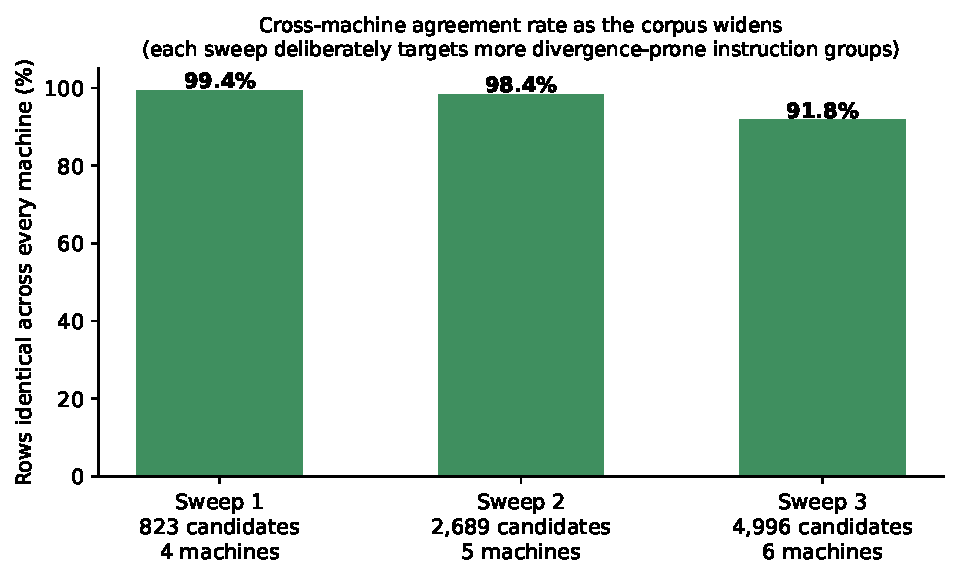
\includegraphics[width=0.75\textwidth]{figures/agreement_rate.pdf}
\caption{Cross-machine agreement rate across the three sweeps. The drop
is a deliberate consequence of corpus design, not increasing noise: each
sweep adds instruction groups chosen specifically because they are more
likely to be generation- or feature-gated.}
\label{fig:agreement}
\end{figure}

In sweep 1 (823 candidates, 4 machines), 818 encodings (99.4\%) agreed on
both length and fault class across every machine. In sweep 2 (2{,}689
candidates under 2 states, 5 machines), 98.4\% agreed. In sweep 3
(4{,}996 candidates, 6 machines), agreement falls to 91.8\%
(Figure~\ref{fig:agreement}). This is the expected and intended result,
not evidence of a noisier harness: sweeps 2 and 3 specifically add the
instruction groups most likely to be generation-gated (AVX-512, AES-NI
variants, PKU, RDRAND/RDSEED, and full group sweeps of reserved ModRM
space), where sweep 1 covered mostly the core one- and two-byte opcode
map, the part of the ISA most heavily validated across implementations.
The falling agreement rate is itself a signal that the corpus is doing
its job: it is finding more of the real divergences reported in
\S\ref{sec:result-crypto} through \S\ref{sec:result-silicon-map} as it
is deliberately pointed at more divergence-prone territory.

\subsection{Resolving the \code{GP\_OR\_PF} Ambiguity}
\label{sec:result-gppf}

\begin{figure}[H]
\centering
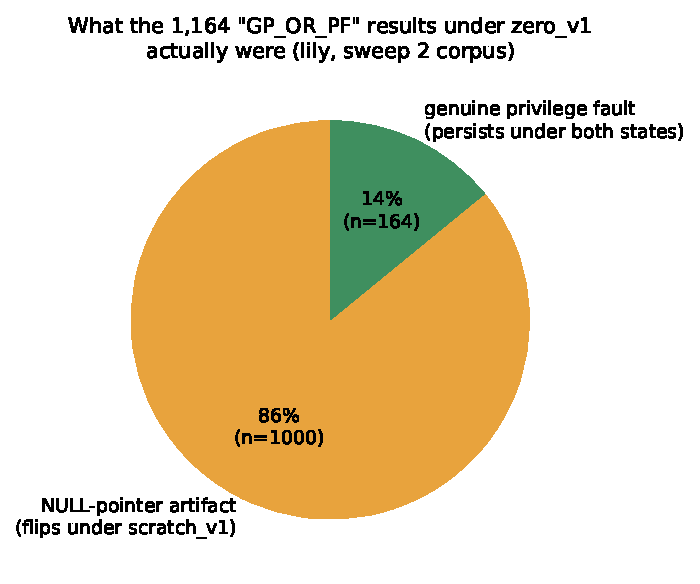
\includegraphics[width=0.6\textwidth]{figures/gppf_breakdown.pdf}
\caption{What the 1{,}164 \code{GP\_OR\_PF} results under \code{zero\_v1}
on lily (sweep 2 corpus) actually were, once compared against the same
candidates under \code{scratch\_v1}.}
\label{fig:gppf}
\end{figure}

Linux reports \code{si\_addr == 0} both for a synthesized \code{\#GP} and
for a genuine \code{\#PF} at a NULL address, so the two are
architecturally indistinguishable from a userspace signal handler alone.
Under \code{zero\_v1}, every GPR is zero, so any ModRM-encoded memory
operand of the form \code{[rax]} dereferences address zero. On lily,
1{,}164 of sweep 2's results were \code{GP\_OR\_PF} under \code{zero\_v1}.
Comparing against the same candidates under \code{scratch\_v1}, where
every GPR points at valid, mapped memory instead, shows that
\textbf{1{,}000 of those 1{,}164 results (86\%) flip to a different fault
class} (Figure~\ref{fig:gppf}): these were incidental NULL-pointer
faults, not genuine privilege detection. The 164 that persist under both
states are the real thing: control and debug register access, MSR
access, I/O-port instructions, and \code{hlt}/\code{cli}/\code{sti}.

This dual-state design turns out to validate itself in an unplanned way,
reported in full in \S\ref{sec:result-security}: for \code{rdpkru} and
\code{wrpkru}, which the SDM requires \code{ECX=0} to execute without
fault, the \emph{same} instructions correctly execute under
\code{zero\_v1} (\code{ECX=0}) and correctly fault under
\code{scratch\_v1} (\code{ECX} nonzero), on exactly the machines that
have PKU at all. The state built to resolve one measurement ambiguity
turned out to also confirm the harness reproduces a documented
operand-validity rule correctly, not only feature presence.

\subsection{Cryptography Acceleration Instructions: the Entry Point, Demonstrated}
\label{sec:result-crypto}

This section is the direct empirical payoff of \S\ref{sec:scope}'s entry
point. Every result below was produced by the same harness and the same
methodology as every other result in this report; nothing here is
cryptography-specific at the tool level, only at the choice of which
bytes were submitted.

\subsubsection{Scalar AES-NI and PCLMULQDQ are universal, and the state-flip confirms it}

\code{aesenc}/\code{aesdec}/\code{aesenclast}/\code{aesdeclast}/
\code{aesimc} (\code{66 0F 38 DB}-\code{DF}) and \code{pclmulqdq}
(\code{66 0F 3A 44}) show \code{GP\_OR\_PF} under \code{zero\_v1} on
\textbf{all six machines}, flipping cleanly to \code{NONE} (clean
execution) under \code{scratch\_v1} on all six.

This was the NULL-deref artifact of \S\ref{sec:result-gppf}, not a
feature gap: scalar AES-NI and PCLMULQDQ have been present on every
machine in this fleet since 2012. This is the baseline the next finding
contrasts against.

\subsubsection{Vectorized AES-NI and PCLMULQDQ are Tiger-Lake-only, confirmed two independent ways}

\code{vaesenc} at VEX.256 width (\code{C4 E2 7D DC}) and
\code{vpclmulqdq} at VEX.256 (\code{C4 E3 7D 44}) show the identical
NULL-deref-then-flip pattern, but only on lily and debian; on the other
four machines they are \code{\#UD} under both states. Table
\ref{tab:avx512}, carried over from the AVX-512-specific sweep, shows
the \emph{same} split a third time through the EVEX-encoded, zmm-width
form of \code{vaesenc}.

A workload that assumes wide AES-GCM throughput because ``AES-NI is
present,'' true on 6/6 machines in this fleet, would be silently wrong
on 4/6 machines the moment it reaches for the vectorized path, and the
SDM alone cannot tell a program which machine it is running on.

\begin{table}[h]
\centering
\caption{AVX-512 seed behavior across the fleet, including the
EVEX-encoded, zmm-width form of AES-NI (\code{vaesenc}). Length is the
engine's empirically resolved instruction length, independent of
validity.}
\label{tab:avx512}
\small
\resizebox{\textwidth}{!}{%
\begin{tabular}{@{}lcccccc@{}}
\toprule
Encoding (instruction) & z420 (SNB-EP) & imac (Haswell) & fuzzarch (KBL-R) & d153 (CFL) & lily (TGL) & debian (TGL) \\
\midrule
\code{62f17c4858c1} (\code{vaddps zmm}) & \#UD, len \textbf{2} & \#UD, len \textbf{2} & \#UD, len 6 & \#UD, len 6 & exec., len 6 & exec., len 6 \\
\code{62f17c48c2c100} (\code{vcmpeqps}) & \#UD, len \textbf{2} & \#UD, len \textbf{2} & \#UD, len 7 & \#UD, len 7 & exec., len 7 & exec., len 7 \\
\code{62f27d4990048f} (\code{vaesenc} zmm) & \#UD, len \textbf{2} & \#UD, len \textbf{2} & \#UD, len 7 & \#UD, len 7 & exec., len 7 & exec., len 7 \\
\bottomrule
\end{tabular}%
}
\end{table}

\subsubsection{RDRAND and RDSEED: a hardware-RNG boundary pinned to the machine, not just the generation}

A full sweep of Group 9 (\code{0F C7}) shows \code{rdrand}
(\code{reg=6}) executes on 5 of 6 machines, \code{\#UD} only on z420
(Sandy Bridge-EP, 2012; RDRAND shipped in Ivy Bridge, 2012, just after).
\code{rdseed} (\code{reg=7}) executes on 4 of 6, \code{\#UD} on z420
\emph{and} imac (Haswell, 2013; RDSEED shipped in Broadwell, 2014).

imac has RDRAND but not RDSEED, landing exactly between the two
features' real introduction dates (Figure~\ref{fig:timeline} makes this
visible directly). Both instructions feed cryptographic key and nonce
generation, making this the clearest single result in the report for a
fine-grained, dated generational boundary rather than a single binary
split.

\subsubsection{SHA-NI and GFNI confirm the same Tiger-Lake-only pattern}

\code{sha256rnds2} (legacy-encoded, no VEX or EVEX needed) and
\code{vgf2p8affineqb} (VEX-encoded; GFNI accelerates the
$\mathrm{GF}(2^8)$ affine transformation at the core of the AES S-box)
both execute only on lily and debian, \code{\#UD} on the other four,
matching the vectorized-AES pattern above through two more, independently
encoded instruction families.

\subsubsection{Gather instructions (Downfall-relevant) follow the AVX-512 decode-generation split exactly}

AVX2 legacy-VEX gather (\code{vpgatherdd}) executes on every machine
that has AVX2 (5 of 6, all but z420). AVX-512 EVEX gather follows the
identical three-tier pattern as every other EVEX-encoded instruction in
this report: executes on Tiger Lake, full-length \code{\#UD} on Kaby
Lake-R/Coffee Lake, and 2-byte-truncated \code{\#UD} on both
pre-EVEX-recognition machines, confirming (\S\ref{sec:result-silicon-map})
that this decoder-level boundary is not a Sandy-Bridge-EP-specific
oddity.

\subsection{Security Mitigations Detected Without Privileged Access}
\label{sec:result-security}

\subsubsection{UMIP}

Three group-selected instructions, \code{sldt} and \code{str}
(\code{0F~00}, ModRM register field 0 and 1) and \code{smsw}
(\code{0F~01}, register field 4), are not architecturally privileged:
the SDM defines all three as executable at any privilege level. They
execute cleanly on four of the six fleet machines and raise \code{\#GP}
in ring~3 on exactly lily and debian, the only two machines with the
\code{umip} CPUID flag, verified independently from
\code{/proc/cpuinfo}. The correspondence is exact in both directions.

\subsubsection{PKU}

The full Group 7 sweep shows \code{rdpkru}/\code{wrpkru}
(\code{0F~01~EE}/\code{EF}) execute cleanly under \code{zero\_v1} on
lily and debian only, \code{\#UD} on the other four, matching
\code{/proc/cpuinfo}'s \code{pku}/\code{ospke} flags exactly
(\S\ref{sec:result-gppf} describes how the dual-state design incidentally
validated this result against the SDM's own \code{ECX=0} requirement).

\subsubsection{Why both findings matter}

UMIP and PKU are not
cryptographic primitives, but they are exactly the kind of fact a
security-sensitive program depends on without being able to check:
whether reading a descriptor-table address from ring 3 is blocked, and
whether a sandboxing scheme built on memory protection keys has real
hardware support, are both facts about the specific chip a program
happens to be running on, not facts the architecture manual settles in
general. The harness recovers both with the same black-box method used
for every result in this report.

\subsection{Beyond Cryptography and Security: a General Silicon Map}
\label{sec:result-silicon-map}

This section is the direct answer to RQ4 and the clearest demonstration
that \project{} is a general-purpose tool. Every figure and finding here
covers instruction groups with no cryptographic or security motivation:
general-purpose SIMD width extensions, memory-ordering and
cache-management instructions, and reserved opcode space.

\begin{figure}[H]
\centering
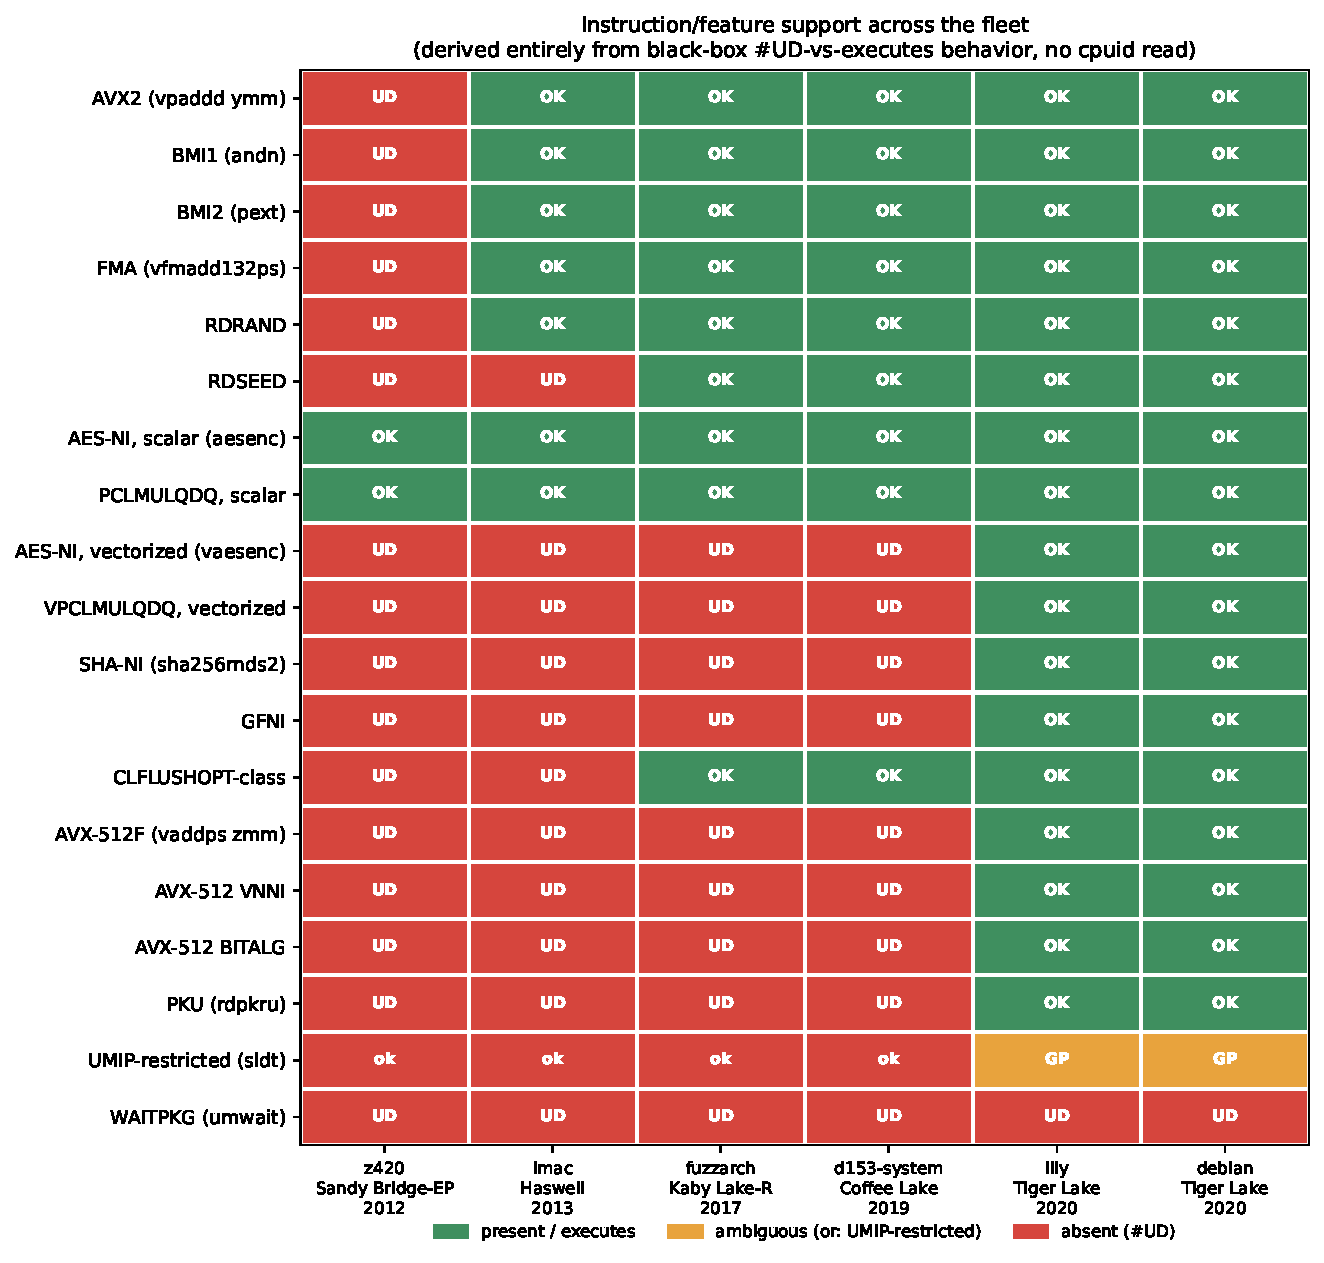
\includegraphics[width=\textwidth]{figures/feature_matrix.pdf}
\caption{Nineteen features across the fleet, derived entirely from
black-box \code{\#UD}-versus-executes behavior under the methodology of
\S\ref{sec:result-gppf}: green is present, red is absent, and the single
orange row (UMIP) is the one feature in this set whose presence is
detected as a \emph{restriction} (\code{\#GP} where the instruction is
otherwise unprivileged) rather than a capability. Nine of the nineteen
rows have nothing to do with cryptography.}
\label{fig:matrix}
\end{figure}

\begin{figure}[H]
\centering
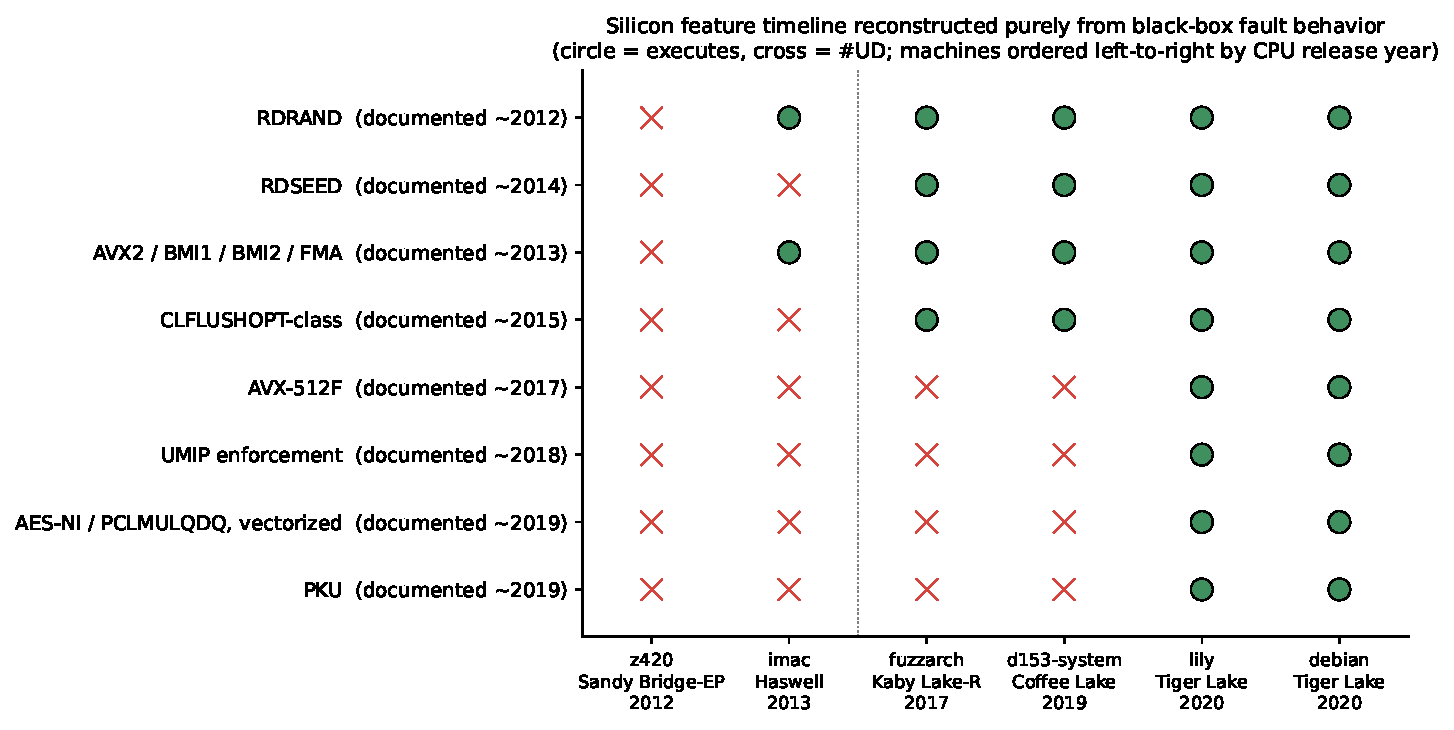
\includegraphics[width=\textwidth]{figures/timeline.pdf}
\caption{Eight features ordered by their documented Intel introduction
generation, plotted against the fleet ordered by CPU release year. The
diagonal-ish boundary between circles (executes) and crosses (\code{\#UD})
is not drawn in; it falls out of the data on its own.}
\label{fig:timeline}
\end{figure}

\subsubsection{The AVX-512 decode-generation split is three-tiered, and the boundary is not where the feature itself was introduced}

Table~\ref{tab:avx512} shows Kaby Lake-R and Coffee Lake decode the
full, correct EVEX length (6--7 bytes) and only then fault, where z420
and imac both truncate to 2 bytes, because their decoders do not
recognize \code{0x62} as an EVEX escape prefix at all and instead read
it as the legacy, 64-bit-mode-invalid \code{BOUND} opcode.

Having a genuine Haswell-generation machine (imac) confirm the same
2-byte truncation as the 2012 Sandy Bridge-EP machine rules out the
possibility that this was a Sandy-Bridge-EP-specific quirk rather than a
real property of pre-EVEX-recognition silicon in general: \code{kmovw},
which is VEX-encoded rather than EVEX-encoded, decodes to its full,
correct length on every machine in the fleet including both of these,
because the VEX prefix format predates all six machines.

\subsubsection{A clean Haswell-generation feature wall, now with the boundary machine itself in the fleet}

BMI1 (\code{andn}), BMI2 (\code{pext}/\code{pdep}), FMA
(\code{vfmadd132ps}), and AVX2 (\code{vpaddd ymm}) execute identically
on all five post-2012 machines, including imac, and \code{\#UD} on
Sandy Bridge-EP alone (Figure~\ref{fig:matrix}). Sweep 2 inferred this
boundary from Sandy Bridge-EP's absence alone; sweep 3 confirms it
directly, since imac is the real Haswell-generation machine where these
features were introduced.

\subsubsection{A CLFLUSHOPT-class boundary around Broadwell}

The \code{66}-prefixed Group 15 sweep shows one ModRM region present on
fuzzarch, d153-system, lily, and debian (Kaby Lake-R and newer) and
\code{\#UD} on z420 and imac (Haswell and older), consistent with
CLFLUSHOPT's real introduction in the Broadwell generation.

\subsubsection{A clean negative control: WAITPKG is absent everywhere}

The \code{F2}-prefixed Group 15 sweep (\code{umwait}/\code{tpause}
territory) is \code{\#UD} on all six machines without exception,
including both Tiger Lake boxes.

This matters methodologically: it shows the technique does not
manufacture a split out of every instruction group it touches. When a
feature genuinely is not present anywhere in the fleet, the method says
so cleanly, which is part of why the splits reported elsewhere in this
section can be trusted.

\subsubsection{A broad decoder-permissiveness shift, reported honestly as an open pattern}

213 of Group 7's 256 ModRM forms are \code{GP\_OR\_PF} on all five newer
machines and \code{\#UD} on z420 alone. This indicates Sandy Bridge-EP's
decoder treats most of this group's undefined encodings as non-existent,
where every newer machine treats the same bytes as existing but
protected.

This report does not attribute each of the 213 forms to a specific
named instruction; that triage is listed as future work
(\S\ref{sec:future}) rather than asserted without verification.

\subsection{A Reproducible Harness Robustness Bug}
\label{sec:result-sigbus}

The sweep-2 corpus crashed the daemon on debian, which runs kernel
7.3.0-rc6+, a pre-release testing kernel. The crash occurs at a specific,
deterministic point: \code{48~9D} (REX.W \code{popfq}) under the
\code{scratch\_v1} state, after roughly 1{,}999 preceding submissions to
that daemon instance. This was investigated with a sequence of controlled
experiments rather than accepted at face value.

A plain sequential replay, using individual \code{submit()} calls with
no batching and no writer thread, reproduces the crash identically. That
rules out a pipe or threading race.

Starting a fresh daemon and running only the \code{scratch\_v1} pass,
without the \code{zero\_v1} pass that normally precedes it, also
reproduces the crash at the same relative point. That rules out
cross-state accumulation.

No segfault or oops shows up in \code{dmesg} or \code{journalctl~-k}, so
this is not a kernel-level crash. The daemon process exits with
Python's reported return code $-7$, meaning it was killed by a raw,
uncaught \code{SIGBUS}, even though \code{signals.c} installs a handler
for that signal. Capturing the daemon's own \code{stderr} across the
crash shows neither the handler's normal result path nor its diagnostic
for a signal arriving outside a controlled attempt; the signal bypassed
the handler entirely.

Submitting \code{48~9D} alone, with no preceding jobs in a fresh daemon,
does not reproduce the crash, which confirms it is a genuine cumulative
effect of roughly 1{,}999 consecutive single-stepped executions in one
process, specific to this kernel version. lily runs the same CPU model,
i7-1165G7, on an older stable kernel, and never shows this behavior.

The sweep-3 corpus, run after the fixes in \S\ref{sec:result-bugs},
completed cleanly on all six machines including debian with no crash at
all, although that is more likely explained by this specific failure
being sensitive to the exact job sequence than by it having been fixed.

The leading hypothesis, documented in \code{docs/safety.md} and not yet
confirmed, is that \code{bx862\_run\_attempt} escapes its own signal
handler through \code{siglongjmp()} rather than a normal handler return,
which skips the kernel's \code{sigreturn} path that would otherwise
restore the process's signal mask. Repeating this roughly 2{,}000 times
in a row, on a kernel whose signal-delivery bookkeeping differs just
enough from a stable kernel on identical hardware, could plausibly leave
\code{SIGBUS} wrongly blocked at the exact moment the CPU raises it
synchronously. The decisive next check, inspecting the \code{SigBlk}
field of \code{/proc/<pid>/status} at the moment of failure, was not
performed for this report.

The engineering response, which should be read as a workaround rather
than a fix, is the function \code{run\_state\_resilient}, added to the
runner script. It auto-reconnects to a fresh daemon on this specific
failure, resumes from the next candidate, recomputes any ASLR-dependent
input state from the new process's own handshake, and logs every
occurrence into the output file's metadata rather than retrying
silently. This produced a complete, 5{,}378-row dataset on debian for
sweep 2, with aggregate fault-class counts matching the other four
machines and exactly one logged crash entry.

% ======================================================================
\section{Discussion}
% ======================================================================

The results build on each other rather than standing as a list of
separate observations.

Sections~\ref{sec:result-correctness} and \ref{sec:result-stability}
establish that the harness is trustworthy: it reproduces a known result
exactly, and its falling cross-machine agreement rate across three
sweeps (Figure~\ref{fig:agreement}) tracks the corpus's deliberate
widening into more divergence-prone territory, not growing noise.

Section~\ref{sec:result-gppf} shows the harness turned on itself: a
plausible-looking privilege-detection signal is shown to be 86\%
measurement artifact (Figure~\ref{fig:gppf}), and the fix, a second
input state implemented in a few lines of Python, is applied, verified,
and later found to validate an unrelated architectural rule (PKU's
\code{ECX=0} requirement) as a side effect.

Section~\ref{sec:result-crypto} delivers on the report's entry point
directly: scalar cryptography acceleration is universal across eight
years of silicon in this fleet, its vectorized counterparts are not,
and the RDRAND/RDSEED boundary is pinned to a specific pair of machines
rather than inferred. Section~\ref{sec:result-security} moves from
cryptography to security proper, recovering two kernel/CPU-enforced
mitigations with the same method.

Section~\ref{sec:result-silicon-map}, anchored by Figures~\ref{fig:matrix}
and \ref{fig:timeline}, is the section that answers RQ4 directly: the
same unmodified harness, pointed at general-purpose SIMD,
memory-ordering, and reserved opcode space with no cryptographic or
security motivation, produces results of the same quality, including a
clean negative control that shows the method is not simply finding a
split in everything it looks at.

Sections~\ref{sec:result-bugs} and \ref{sec:result-sigbus} are included
on purpose rather than as filler. All three safety findings describe
cases where the harness, running at scale against real heterogeneous
machines, exposed its own defects; two were isolated with controlled
experiments and fixed outright, and the third was isolated just as
carefully and reported as open rather than forced into a fix the
evidence did not support. That is the same empirical discipline the
project applies to the silicon it studies, applied here to its own
tooling.

% ======================================================================
\section{Limitations and Threats to Validity}
\label{sec:limitations}
% ======================================================================

\begin{itemize}
  \item \textbf{No reference decoder.} XED and liblisa, called for in
    the project's long-term design, are not wired in yet. Every length
    and fault claim in this report is an empirical, cross-machine
    comparison, not a comparison against documented ground truth. The
    8.2\% of divergent rows in sweep 3 that are not individually
    attributed to a named feature in this report, including the 213-row
    Group 7 pattern in \S\ref{sec:result-silicon-map}, have not been
    triaged byte-by-byte against the SDM. Some may be further real
    findings; others may be corpus artifacts.
  \item \textbf{No microcode-revision walk.} The project's planned
    Idea~1, walking microcode revisions on one machine to detect
    update-induced ISA drift, has not been attempted. Every comparison
    in this report is cross-machine, not cross-revision on fixed
    silicon.
  \item \textbf{No ring-0 or MSR-level work.} Everything in this report
    is ring-3. The sacrificial Xeon (z420) was used only in its safe,
    ring-3 mode. No privileged or MSR-search experiments, the project's
    planned Ideas~4 and~5, have been attempted on it or anywhere else.
  \item \textbf{The SIGBUS finding (\S\ref{sec:result-sigbus}) is
    characterized but not root-caused.} The signal-mask-leak hypothesis
    is consistent with every controlled experiment performed so far, but
    it has not been confirmed by direct inspection of the process's
    signal mask at the moment of failure, and it did not reproduce at
    all during sweep 3, which weakens confidence in any explanation that
    predicts it should recur deterministically.
  \item \textbf{The feature matrix (Figure~\ref{fig:matrix}) uses one
    representative encoding per feature family,} not an exhaustive sweep
    of every encoding variant for every feature (AVX-512 alone has many
    sub-extensions beyond the four sampled here). It is a map of the
    features this corpus specifically probed, not a complete CPUID
    leaf-by-leaf audit.
  \item \textbf{Corpus coverage is intentionally not exhaustive.} 4{,}996
    candidates cover a much larger but still partial fraction of the
    full multi-byte x86 encoding space. Full ModRM/SIB sweeps exist for
    only a handful of group-coded opcodes (\code{0F~01}, \code{0F~AE}
    under four prefixes, \code{0F~C7}); most others are sampled by reg
    field only. Claims of agreement or divergence in this report are
    claims about this corpus, not about the full ISA.
\end{itemize}

% ======================================================================
\section{Future Work}
\label{sec:future}
% ======================================================================

\begin{enumerate}
  \item Integrate XED as a reference oracle, replacing the best-effort
    byte-pattern blacklist with real ModRM/SIB-aware decoding, and
    enabling automatic divergence flagging against documented semantics
    for the full corpus rather than only the named seeds, including
    triaging the 213-row Group 7 pattern from
    \S\ref{sec:result-silicon-map} byte by byte.
  \item Carry out Idea~1, the microcode-revision walk: stage sequential
    microcode blobs for one CPU model and re-run the full corpus after
    each late load, to separate cross-machine drift, which is what this
    report measures, from cross-revision drift on fixed silicon.
  \item Build the ring-0 backends planned as Ideas~4 and~5: a KVM-guest
    ring-0 backend first, which keeps the host safe while virtualizing
    privileged execution, then a bare-metal bootable injector on z420
    specifically, with IPMI- or watchdog-based automatic recovery, to
    study privileged and MSR-gated behavior that is architecturally
    invisible from ring~3.
  \item Extend the security-posture fingerprinting of
    \S\ref{sec:result-security} systematically: enumerate other
    \code{CR4}-gated and \code{IA32\_ARCH\_CAPABILITIES}-gated behaviors
    beyond UMIP and PKU, such as SMAP, SMEP where ring-3-observable, and
    CET/shadow-stack enforcement, and test whether each can be recovered
    the same way.
  \item Extend Figure~\ref{fig:matrix} to a full CPUID leaf audit:
    sample every documented AVX-512 sub-extension and every other
    feature-gated instruction family systematically, rather than one
    representative encoding per family as in this report.
  \item Root-cause the SIGBUS finding from \S\ref{sec:result-sigbus} by
    inspecting \code{/proc/<pid>/status}'s \code{SigBlk} field at the
    instant of failure, and by auditing every \code{siglongjmp} exit
    path in \code{signals.c} for missing signal-mask restoration.
\end{enumerate}

% ======================================================================
\section{Conclusion}
% ======================================================================

This report opened with a claim from the security literature that a
cryptographic algorithm's correctness says nothing on its own about the
security of a system built around it \cite{anderson1993, kocher1996,
schneier1998}, and with the observation that the hardware underneath
every such system is a black box whose documentation describes intended
behavior without being able to guarantee it \cite{thompson1984,
king2008, becker2013, kocher2019spectre, lipp2018meltdown,
moghimi2023downfall}. It then stated explicitly, in \S\ref{sec:scope},
that cryptography would be the entry point into this problem and not
its boundary, because the tool built to study it, \project{}, is a
general-purpose black-box instruction fuzzer, not a cryptography-specific
checker.

The results bear that scope out. Sections~\ref{sec:result-crypto} and
\ref{sec:result-security} deliver the entry point directly: scalar
AES-NI and PCLMULQDQ are confirmed universal across eight years of this
fleet's silicon, their vectorized counterparts and the RDRAND/RDSEED
hardware-RNG boundary are pinned to specific machines rather than
inferred, and UMIP and PKU, two kernel/CPU-enforced security
mitigations, are detected from fault behavior alone.

Section~\ref{sec:result-silicon-map}, built on Figures~\ref{fig:matrix}
and \ref{fig:timeline}, then shows the identical method, with no
redesign, recovering a 19-feature map and an 8-feature generational
timeline across instruction groups that have nothing to do with
cryptography, including a clean negative control that shows the method
does not manufacture divergence where none exists.

Three real engineering defects in the harness itself were found during
this work, two fixed outright and regression-tested, one characterized
through controlled experiments and reported honestly as unresolved,
which is evidence that the project's empirical discipline applies to its
own tooling and not only to the silicon under study.

Taken together, these results support the report's opening claim rather
than merely illustrating it: what a given piece of silicon will
actually do, cryptographically, securely, or otherwise, is a fact about
that silicon, not a fact that follows from reading the manual it shipped
with, and that fact can be recovered, at increasing scale and across an
increasing fleet, without any special access to the chip.

% ======================================================================
\appendix
\section{Reproducibility}
\label{app:repro}
% ======================================================================

Every number and figure in this report can be reproduced from the
\project{} codebase, published at
\url{https://github.com/vajradevam/veritas86}, using the commands
below.

\begin{lstlisting}[style=hex]
# Build and verify the engine (per machine):
make -C core/injector && make -C core/tests
./scripts/safety_preflight.sh && ./core/tests/smoke
python3 -m pytest orchestrator/tests -q

# Run the full sweep (writes data/fingerprints/<hostname>.jsonl):
cd orchestrator && python3 -m tsfuzz.runner

# Cross-machine diff (reads any number of .jsonl files; still from orchestrator/):
python3 -m tsfuzz.diff ../data/fingerprints/*.jsonl
\end{lstlisting}

Raw per-machine fingerprint data for the sweep reported in full here
(sweep 3) lives in \texttt{data/fingerprints/}, one file per host:
\texttt{z420.jsonl}, \texttt{imac.jsonl}, \texttt{fuzzarch.jsonl},
\texttt{d153-system.jsonl}, \texttt{lily.jsonl}, and
\texttt{debian.jsonl}. Each has 9{,}992 rows, one JSON object per line,
and the first line holds the run's identity and provenance block.

Full diff output is in \texttt{data/reports/sweep3\_diff.txt}; earlier
sweeps' data and diffs are kept alongside it as
\texttt{sweep1\_*}/\texttt{sweep2\_*}. The narrative write-ups this
report draws from are \texttt{data/reports/sweep1\_results.md} and
\texttt{data/reports/sweep3\_results.md}. Harness-safety notes,
including all three blacklist fixes and the full SIGBUS investigation,
are in \texttt{docs/safety.md}. The figures in this report were
generated directly from the sweep-3 \texttt{.jsonl} files; the
generating script is kept alongside this report's source.

\begin{thebibliography}{99}

\bibitem{domas2017}
Christopher Domas.
\emph{Breaking the x86 Instruction Set}.
Black Hat USA, 2017.
(Whitepaper included in this project's repository root;
project also known as \emph{sandsifter}.)

\bibitem{intelsdm}
Intel Corporation.
\emph{Intel\textsuperscript{\textregistered} 64 and IA-32 Architectures
Software Developer's Manual}, Volume 3 (System Programming Guide),
\S2.5 (Control Registers) for \code{CR4.UMIP} and the Protection Keys
chapter for \code{RDPKRU}/\code{WRPKRU}.

\bibitem{anderson1993}
Ross Anderson.
Why Cryptosystems Fail.
\emph{Proceedings of the 1st ACM Conference on Computer and
Communications Security (CCS)}, 1993.

\bibitem{kocher1996}
Paul C. Kocher.
Timing Attacks on Implementations of Diffie-Hellman, RSA, DSS, and Other
Systems.
\emph{Advances in Cryptology: CRYPTO '96}, Lecture Notes in Computer
Science, vol. 1109, Springer, 1996.

\bibitem{schneier1998}
Bruce Schneier.
Security Pitfalls in Cryptography.
Counterpane Systems whitepaper, 1998.

\bibitem{thompson1984}
Ken Thompson.
Reflections on Trusting Trust.
\emph{Communications of the ACM}, 27(8), 1984. (1983 ACM Turing Award
lecture.)

\bibitem{king2008}
Samuel T. King, Joseph Tucek, Anthony Cozzie, Chris Grier, Weihang Jiang,
and Yuanyuan Zhou.
Designing and Implementing Malicious Hardware.
\emph{Proceedings of the 1st USENIX Workshop on Large-Scale Exploits and
Emergent Threats (LEET)}, 2008.

\bibitem{becker2013}
Georg T. Becker, Francesco Regazzoni, Christof Paar, and Wayne P. Burleson.
Stealthy Dopant-Level Hardware Trojans.
\emph{Cryptographic Hardware and Embedded Systems (CHES)}, Lecture Notes
in Computer Science, vol. 8086, Springer, 2013.

\bibitem{kocher2019spectre}
Paul Kocher, Jann Horn, Anders Fogh, Daniel Genkin, Daniel Gruss, Werner
Haas, Mike Hamburg, Moritz Lipp, Stefan Mangard, Thomas Prescher, Michael
Schwarz, and Yuval Yarom.
Spectre Attacks: Exploiting Speculative Execution.
\emph{IEEE Symposium on Security and Privacy (S\&P)}, 2019.

\bibitem{lipp2018meltdown}
Moritz Lipp, Michael Schwarz, Daniel Gruss, Thomas Prescher, Werner Haas,
Anders Fogh, Jann Horn, Stefan Mangard, Paul Kocher, Daniel Genkin, Yuval
Yarom, and Mike Hamburg.
Meltdown: Reading Kernel Memory from User Space.
\emph{27th USENIX Security Symposium}, 2018.

\bibitem{moghimi2023downfall}
Daniel Moghimi.
Downfall: Exploiting Speculative Data Gathering.
\emph{32nd USENIX Security Symposium}, 2023.

\end{thebibliography}

\end{document}
